\documentclass[10pt]{article}

\usepackage{fullpage}

\usepackage{tikz}

\usetikzlibrary{shapes.geometric, arrows}

\setlength{\parindent}{0pt}

\tikzstyle{boxEmulate} = [rectangle, rounded corners,  text width=1.9cm, minimum width=2cm, minimum height=1cm, text centered, draw=black, fill=white]

\tikzstyle{boxUtils} = [rectangle, rounded corners,  text width=6cm, minimum width=3cm, minimum height=1cm, draw=black, fill=white]

\tikzstyle{arrow} = [thick, ->, >=stealth]

\begin{document}

\title{FINAL REPORT}
\date{}
\author{Sanchit, Morkus, Luqman,  Alex}

\maketitle

\section*{Introduction}


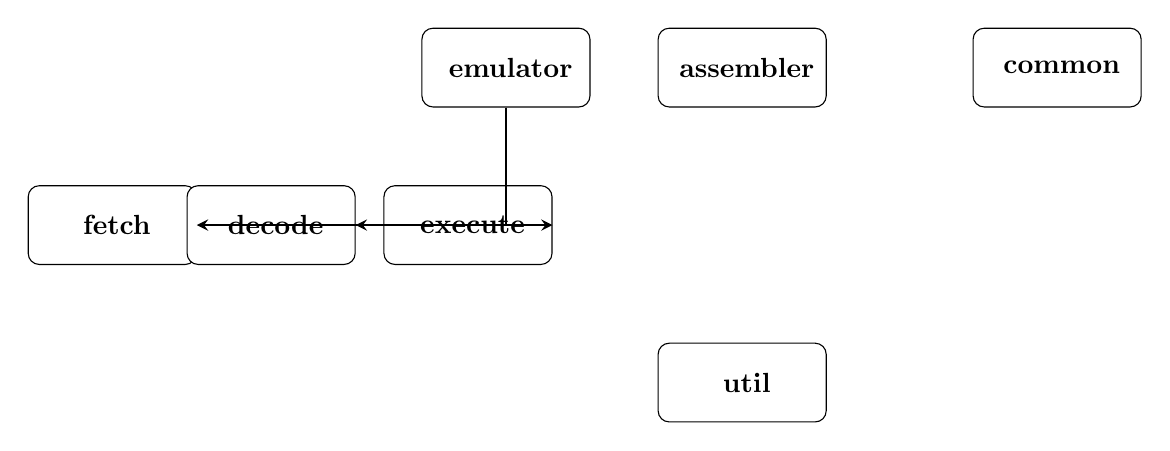
\begin{tikzpicture}[node distance=2cm]

\node (emulator) [boxEmulate, xshift = 5cm] {
\textbf{ emulator} 
};

\node (fetch) [boxEmulate, yshift = -2cm] {
\textbf{ fetch} 

};

\node (decode) [boxEmulate, xshift=0.5, right of= fetch ] {
\textbf{ decode} 

};

\node (execute) [boxEmulate, right of = decode, xshift = 0.5cm] {
\textbf{ execute} 

};



\node (assembler) [boxEmulate, right of = emulator, xshift = 1cm] {
\textbf{ assembler} 

};

\node (util) [boxEmulate, yshift = -4cm, xshift = 8cm] {
\textbf{ util} 

};

\node (common) [boxEmulate, right of = assembler, xshift = 2cm] {
\textbf{ common} 

};

\draw[arrow] (emulator.south) |-(decode);
\draw[arrow] (emulator.south) |-(execute);
\draw[arrow] (emulator.south) |-(fetch);




\end{tikzpicture}
\end{document}